\section{tree\_map\_for\_sequence} \label{sec-treemapseq}

This tools allows you to find a certain sequence in a Newick tree. This
tool creates a \emph{map} file that you can use in conjunction with the
Newick utilities \cite{newick_tools} published by the University of Geneva, in
order to highlight clusters in different colors that contain a
sequence in question.

\subsection{Usage}

The \emph{tree\_map\_for\_sequence} tool can be used:
\lstset{language=bash,
  caption={Calling the \emph{tree\_map\_for\_sequence} tool},
  label=lst-treemapseq-call}
\begin{lstlisting}
tree_map_for_sequence [fasta-ds] [fasta-seq] [color] [split-sets] > [map]
\end{lstlisting}
with the following arguments:
\begin{enumerate}
  \item \emph{fasta-ds} A FASTA file containing the full dataset of
    that has been used to perform an adaptive clustering run with the
    tools shown in section \ref{sec-adaptive-clust}.
  \item \emph{fasta-seq} A FASTA file containing the single sequence
    to be outlined in a Newick tree by using this tool in conjunction
    with the Newick utilities.
  \item \emph{color} A string telling which color to use to mark
    clusters that contains the sequence in question. The color has to
    be expressed in a Cascade Style Sheet (CSS) compatible way. Hence
    simple color expressions such as red, green and blue should
    work. In general it is preferred to use colors in the format
    \#RRGGBB where lead by a hash and three hexadecimal numbers for the
    color values of red, green and blue are used. Hence in order to
    get an orange color you might use, \#FF8800 which corresponds to
    full red, about half green and no blue. 
  \item \emph{split-sets} All the binary clusterings that built the
    tree. And that were used when running the
    \emph{split\_sets\_to\_newick} tool, outlined in section
    \ref{sec-ssnewick}, in order to generate the
    dendogram that the tree visualization using the Newick tools will
    use finally.
  \item \emph{map}
    The resulting \emph{map} file that can be used together with the
    Newick utilities to generate a tree where all clusters containing
    a specific sequence are colored.
\end{enumerate}

\subsection{Example}
\lstset{language=bash,
  caption={Example of the \emph{tree\_map\_for\_sequence} tool},
  label=lst-treemapseq-example}
\begin{lstlisting}
tree_map_for_sequence test.fasta seq.fasta '#FF0000' /tmp/s* > tree.map
\end{lstlisting}
In this example we generate a map file \emph{tree.map} to color all
clusters that contain the sequence contained in \emph{seq.fasta} red in a
tree that we print using the Newick utilities. The tree was built from
the complete dataset of sequences found in \emph{test.fasta}. The
binary \emph{split-sets} that build the different layers of the tree
are found at \emph{/tmp/sX} where $X$ is the number of each layer. And
as with all the previous tools the wild card selection should work
perfectly. To better illustrate the usage of the tool we show in the
following in concordance with the the \emph{split\_sets\_to\_newick}
found in section \ref{sec-ssnewick}, and the Newick utilities
\cite{newick_tools} by the university of Geneva.
\lstset{language=bash,
  caption={Further example of the \emph{tree\_map\_for\_sequence} tool},
  label=lst-treemapseq-example-extended}
\begin{lstlisting}
split_sets_to_newick 0 test.fasta 0 /tmp/s* > tree.dnd
tree_map_for_sequence test.fasta seq.fasta '#FF0000' /tmp/s* > tree.map
nw_display -w 600 -rs -i 'opacity:0' -b 'opacity:0' -l 'opacity:0' \
  -c tree.map tree.dnd > tree.svg
\end{lstlisting}
where \emph{tree.dnd} is the Newick file that corresponds to the map
\emph{tree.map} that we generate with the tool outlined in this
section. The \emph{nw\_display} from the Newick utilities
\cite{newick_tools} generates an svg image without annotations of a
with of 600 points in radial fashion. It uses the aforementioned map
to color clusters in the tree red that contain the sequence in
question. An example tree generated like this is shown in figure
\ref{fig-treemapseq}.

\begin{figure}
  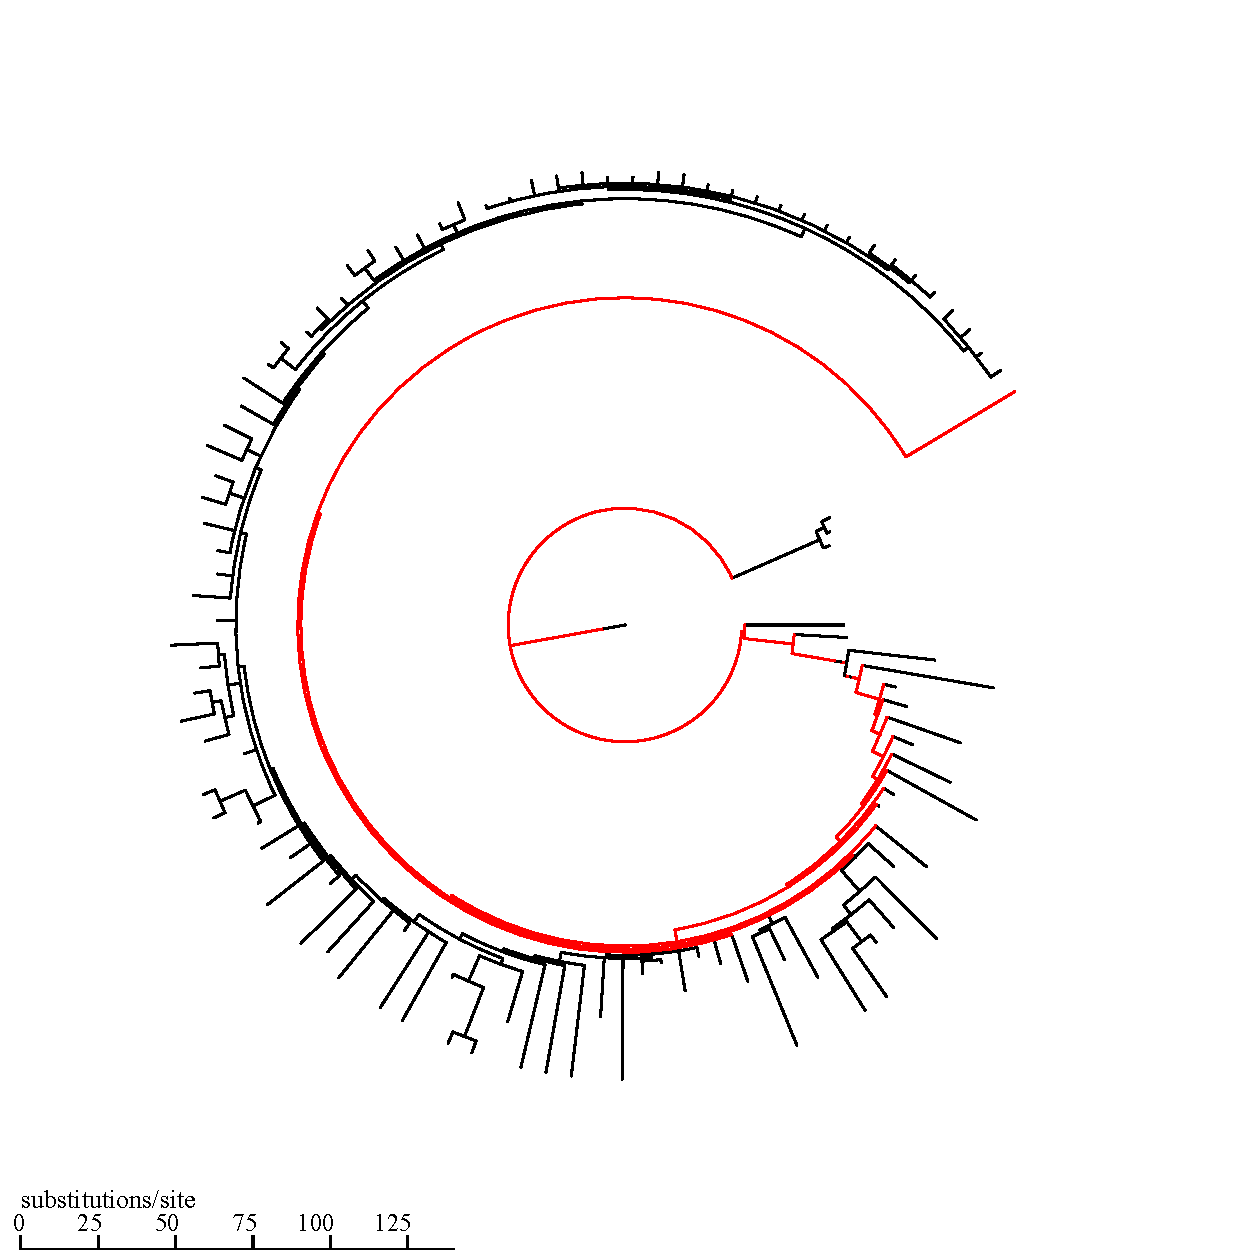
\includegraphics[scale=0.7]{tree-stroke.pdf}
  \caption{An example of a tree that outlines with a red line the
    location of a certain sequence. A tree generated using the tools in
    order as outlined in listing
    \ref{lst-treemapseq-example-extended}. The substitutions/site
    scale automatically generated by the Newick utilities
    \cite{newick_tools} can be ignored.}
  \label{fig-treemapseq}
\end{figure}

\subsection{Implementation}
The \emph{tree\_map\_for\_sequence} tool is implemented in \newline
\emph{tree\_map\_for\_sequence.c}.

